%******************************************************************************%
%                                                                              %
%                  JavaScript.en.tex for LaTeX                                 %
%                  Created on : Tue Mar 10 13:27:28 2015                       %
%                  Made by : Don Stolz <dstolz@student.42.us.org>              %
%                                                                              %
%******************************************************************************%

\documentclass{42-en}


%******************************************************************************%
%                                                                              %
%                                    Header                                    %
%                                                                              %
%******************************************************************************%
\begin{document}
\title{JavaScript}
\member{Donald Stolz}{dstolz@student.42.us.org}
\summary {
 Setup a MongoDB cloud account and cluster. 
}
\maketitle

\tableofcontents

%******************************************************************************%
%                                                                              %
%                                 Introduction                                 %
%                                                                              %
%******************************************************************************%
\chapter{Introduction}

Follow these instructions to setup MongoDB.

%******************************************************************************%
%                                                                              %
%                                  Instructions                                %
%                                                                              %
%******************************************************************************%
\chapter{Instructions}

First head to \href{https://www.mongodb.com/}{https://www.mongodb.com/}

\begin{figure}[H]
    \begin{center}
        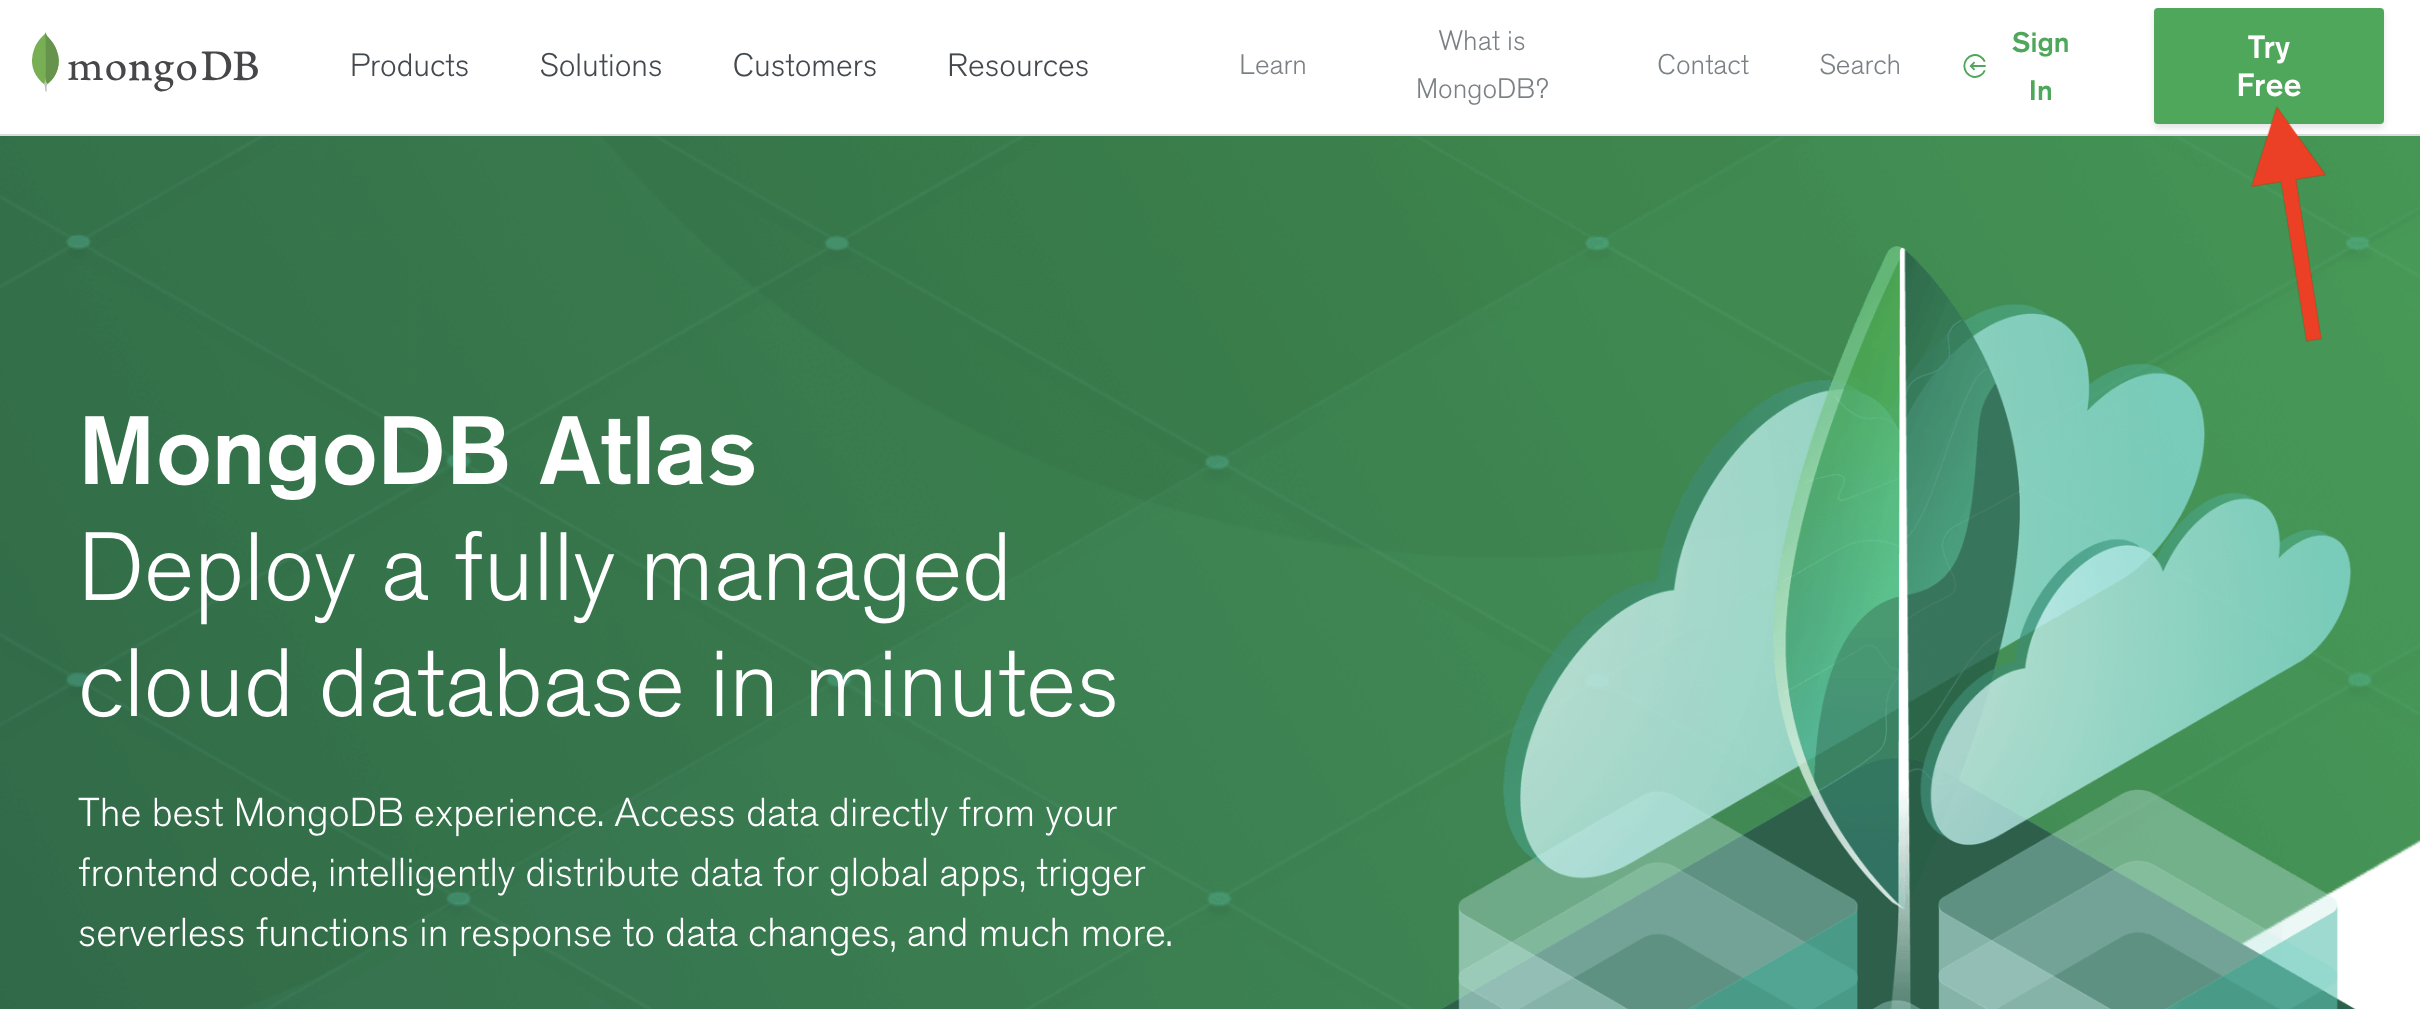
\includegraphics[width=14cm]{WEB/mongo_0.png}
    \end{center}
\end{figure}

Fill out the simple form to create an account
\begin{figure}[H]
    \begin{center}
        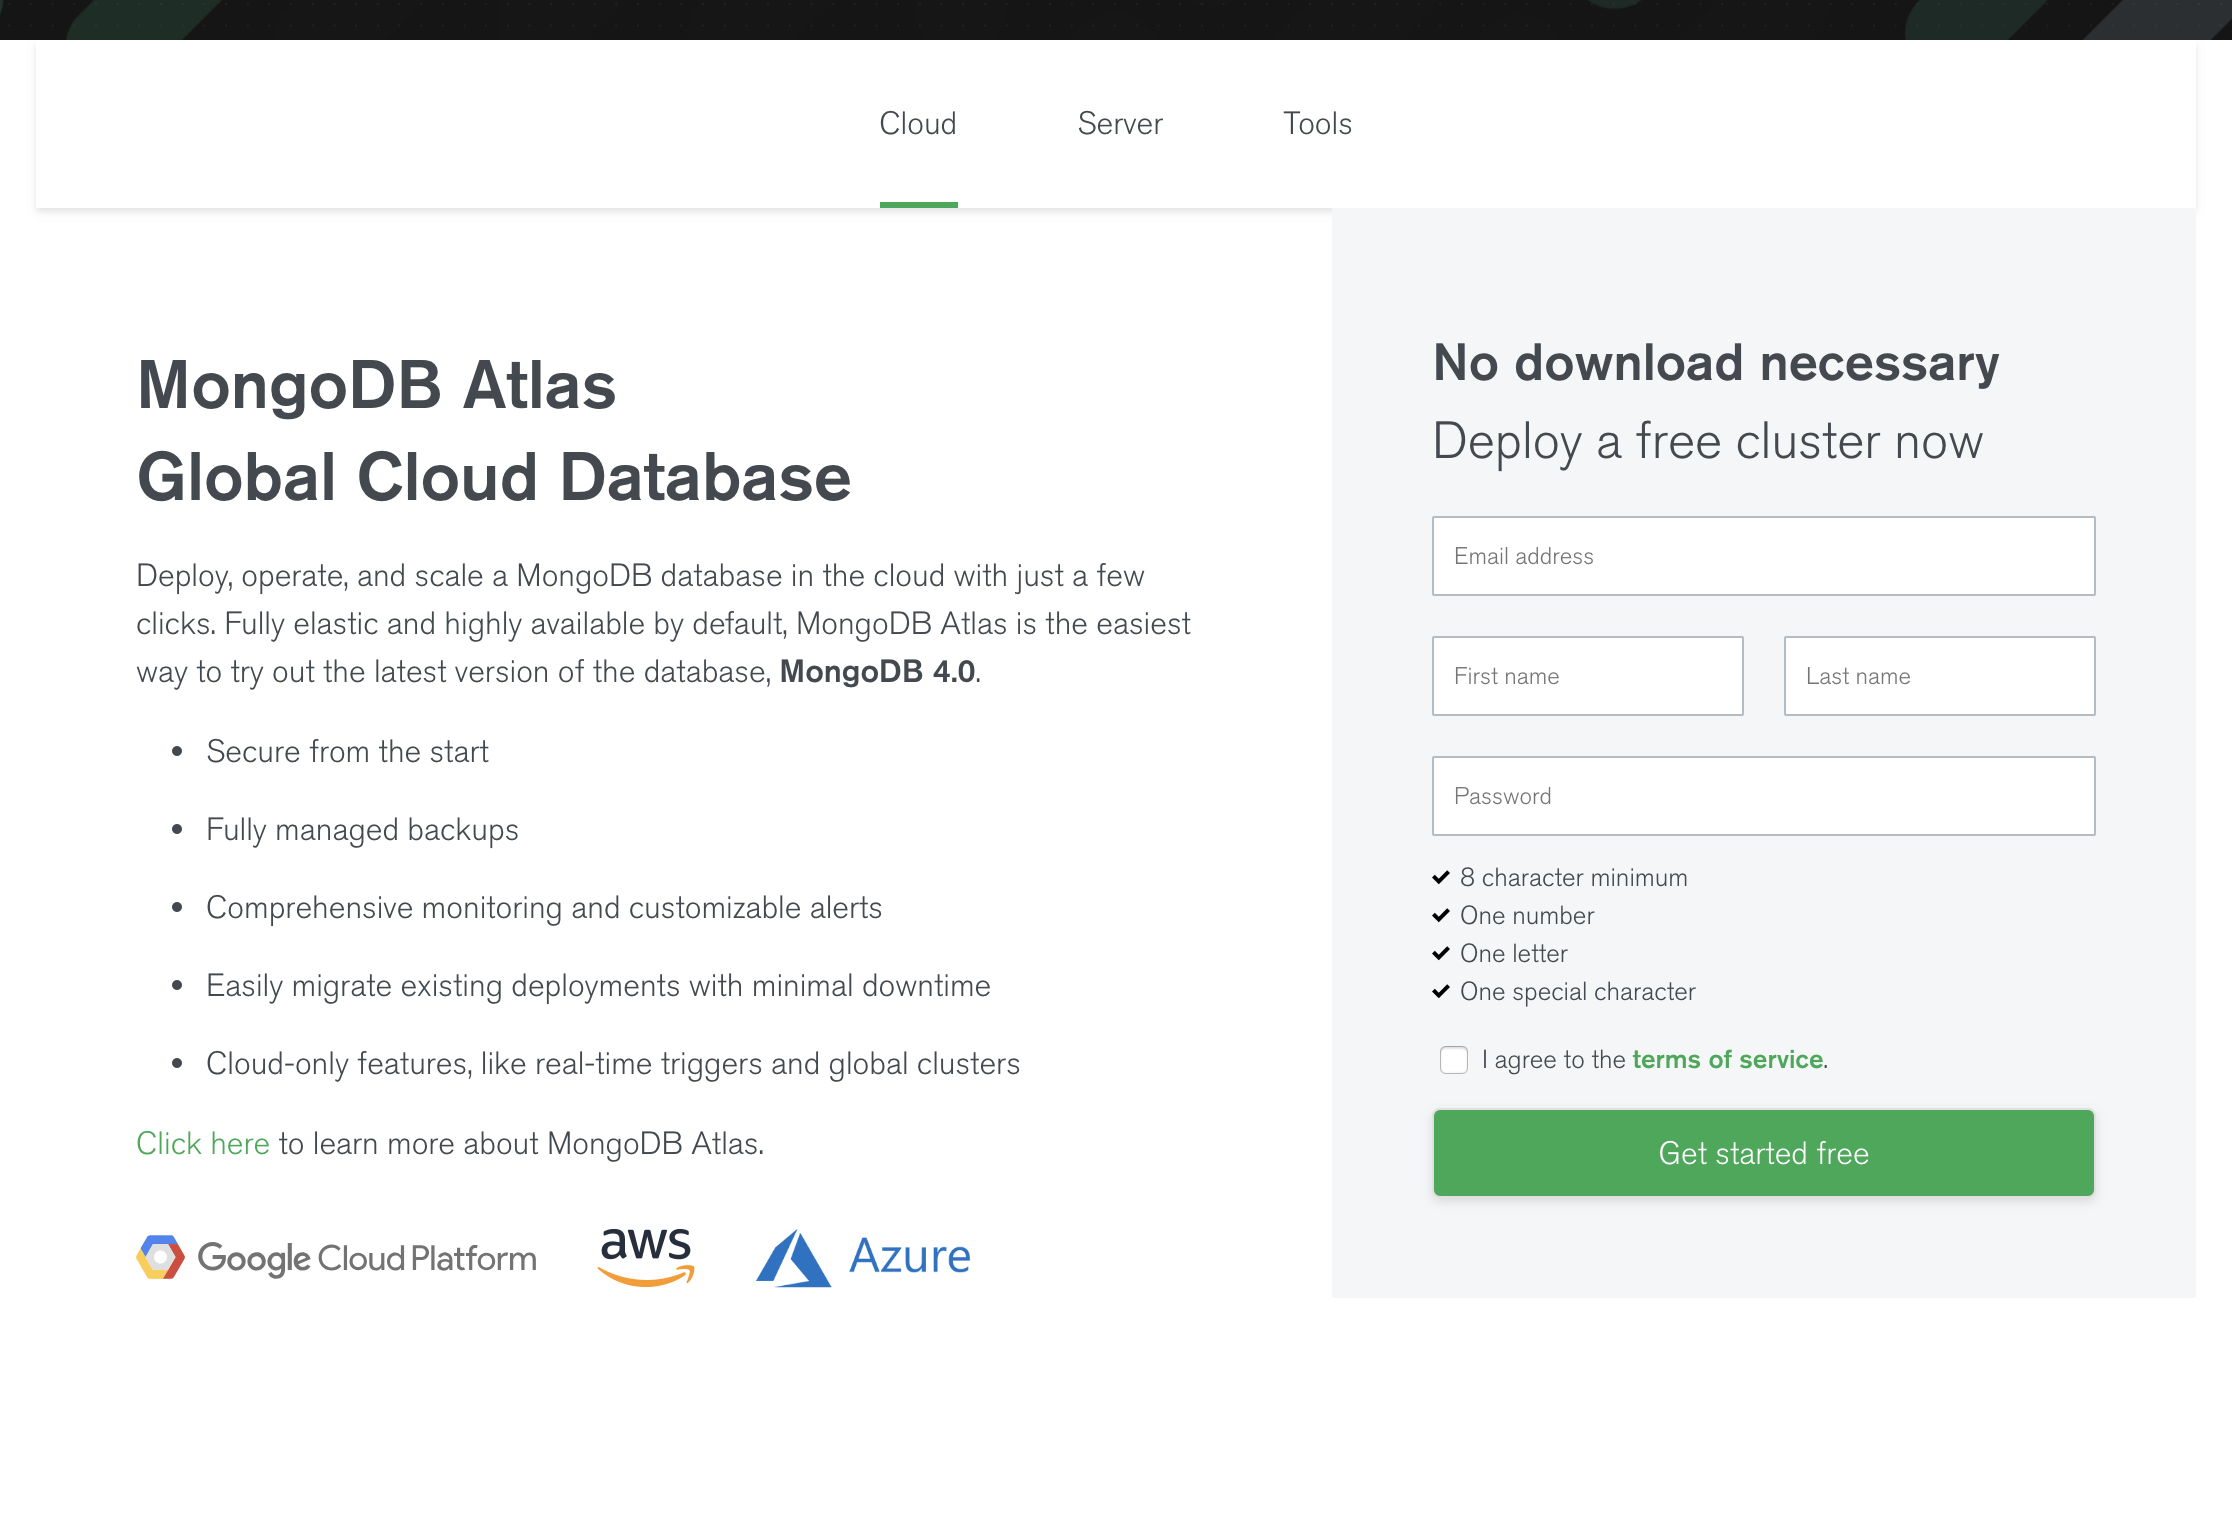
\includegraphics[width=14cm]{WEB/mongo_1.png}
    \end{center}
\end{figure}

\newpage
Once you start creating a new cluster the only piece of the form you should change is the Cluster Name, at the bottom
\begin{figure}[H]
    \begin{center}
        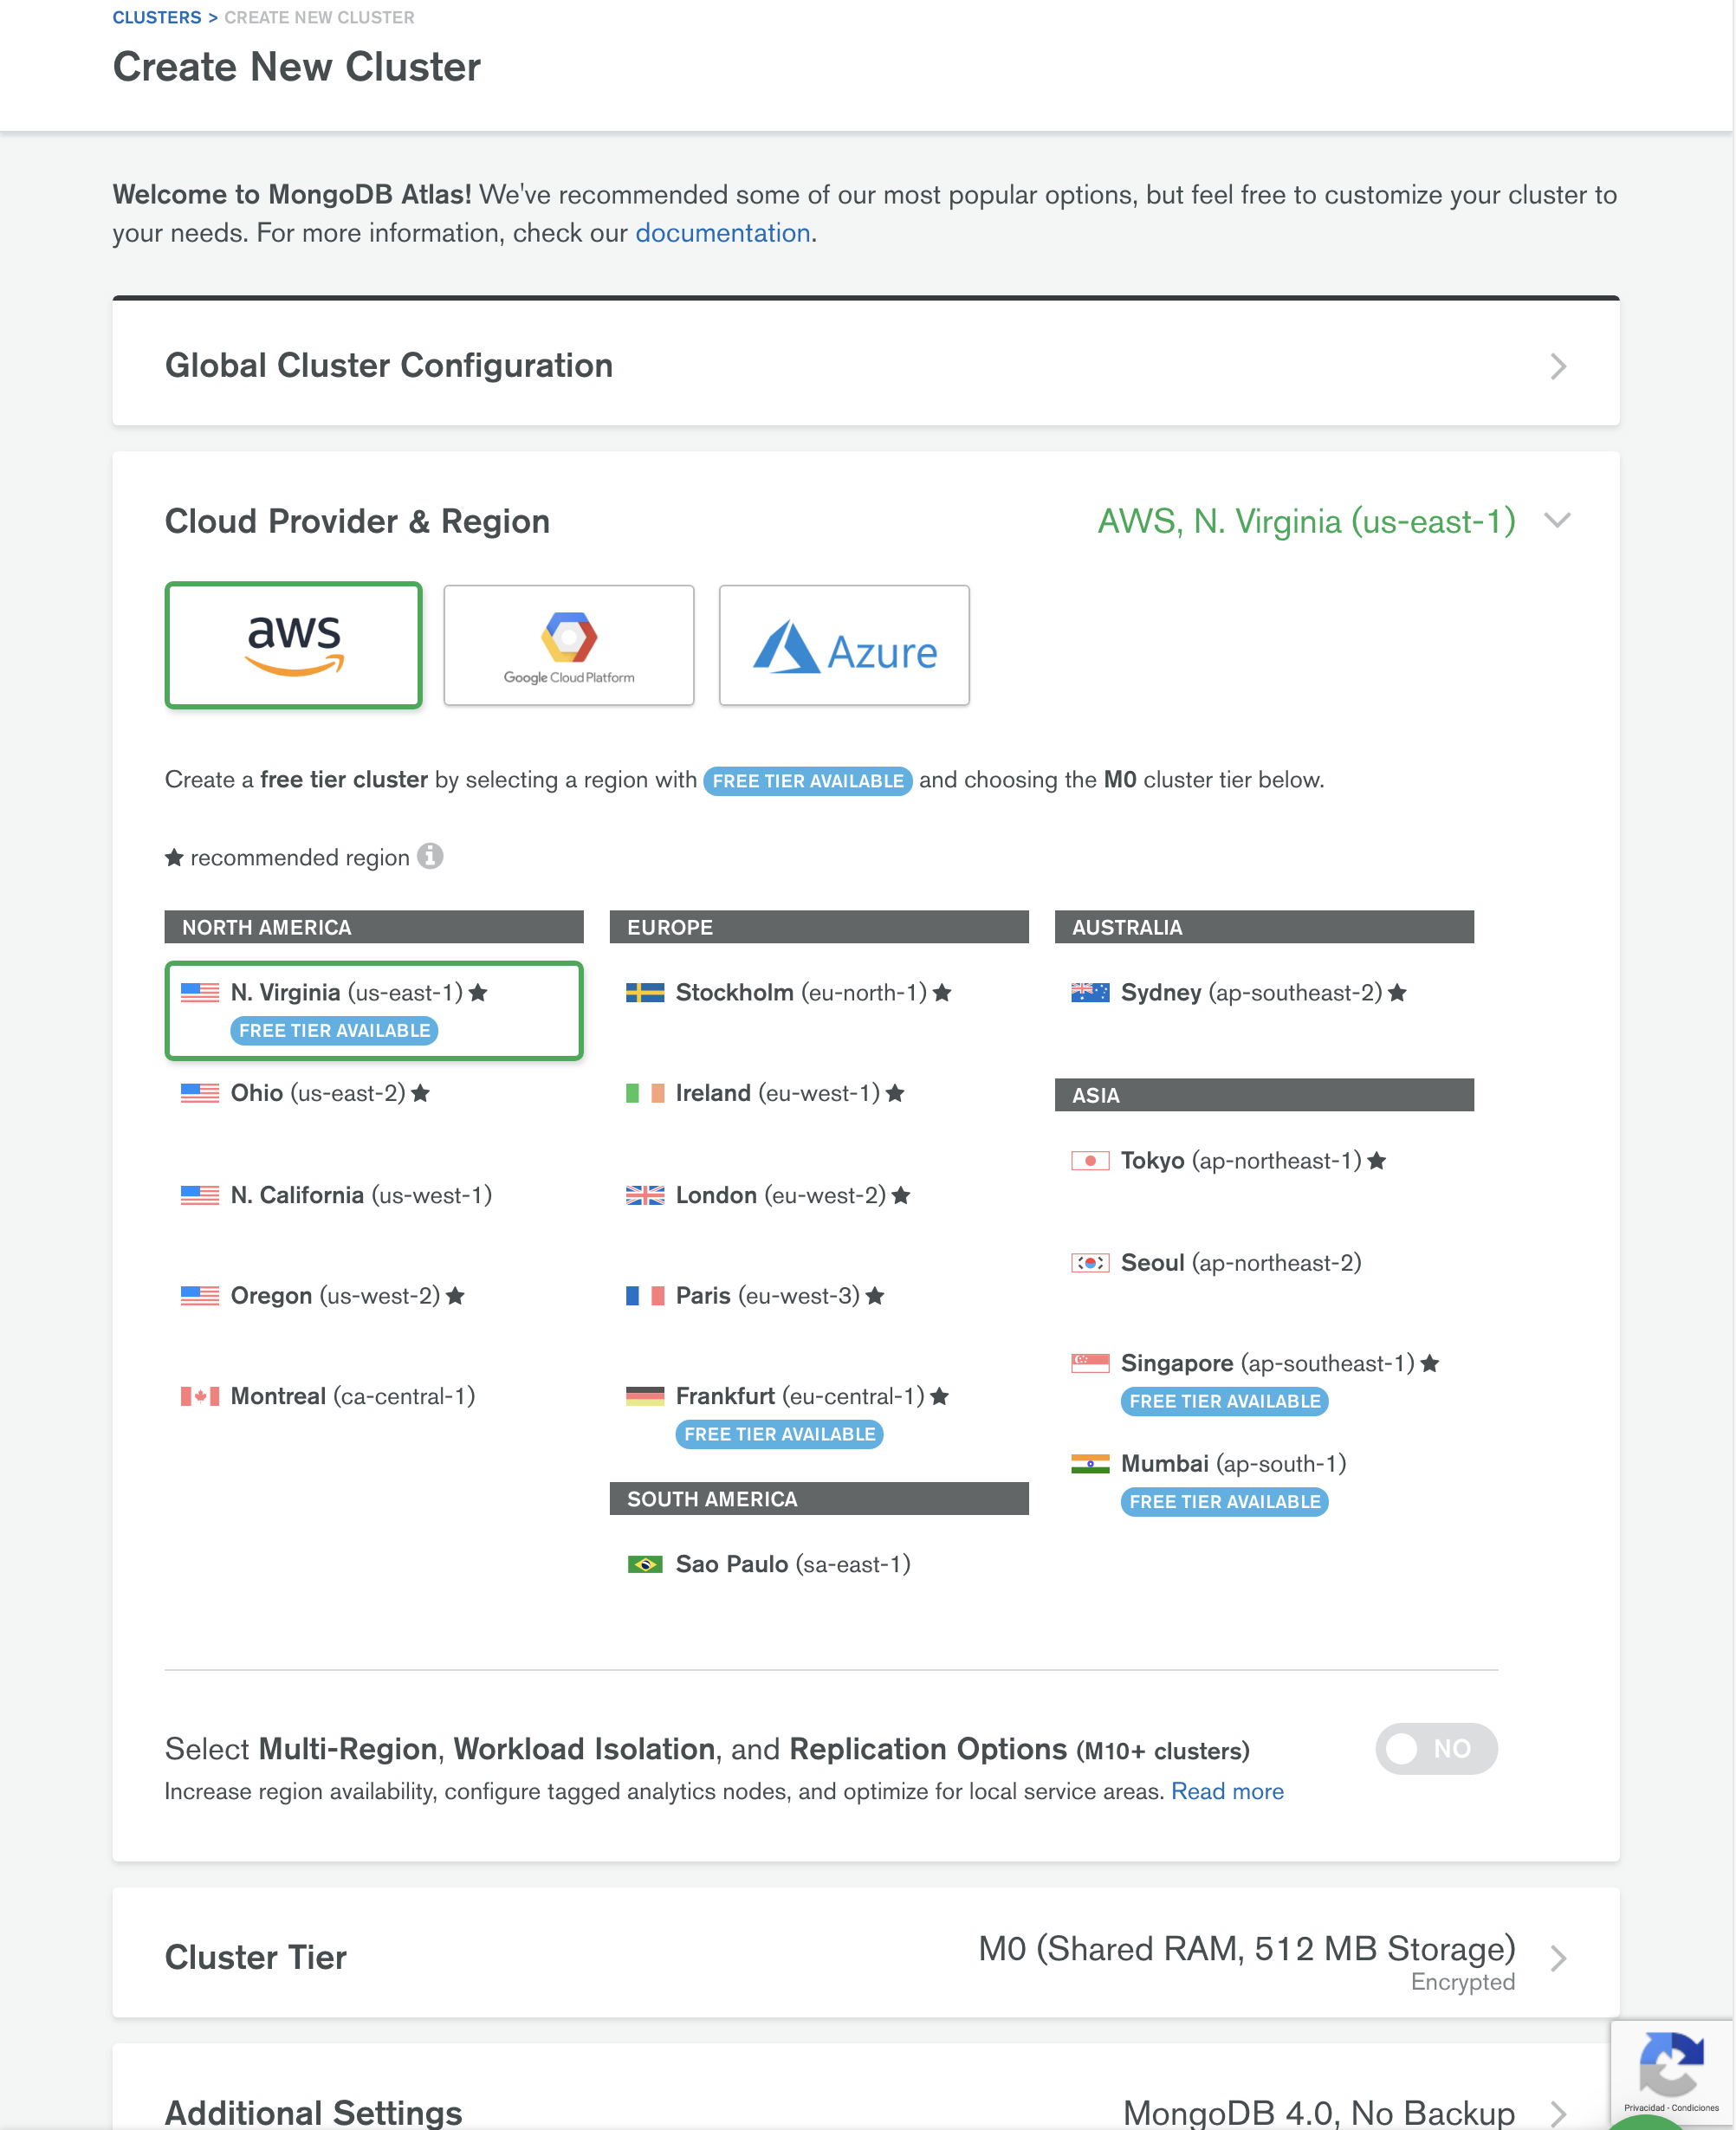
\includegraphics[width=12cm]{WEB/mongo_2.png}
    \end{center}
\end{figure}

\begin{figure}[H]
    \begin{center}
        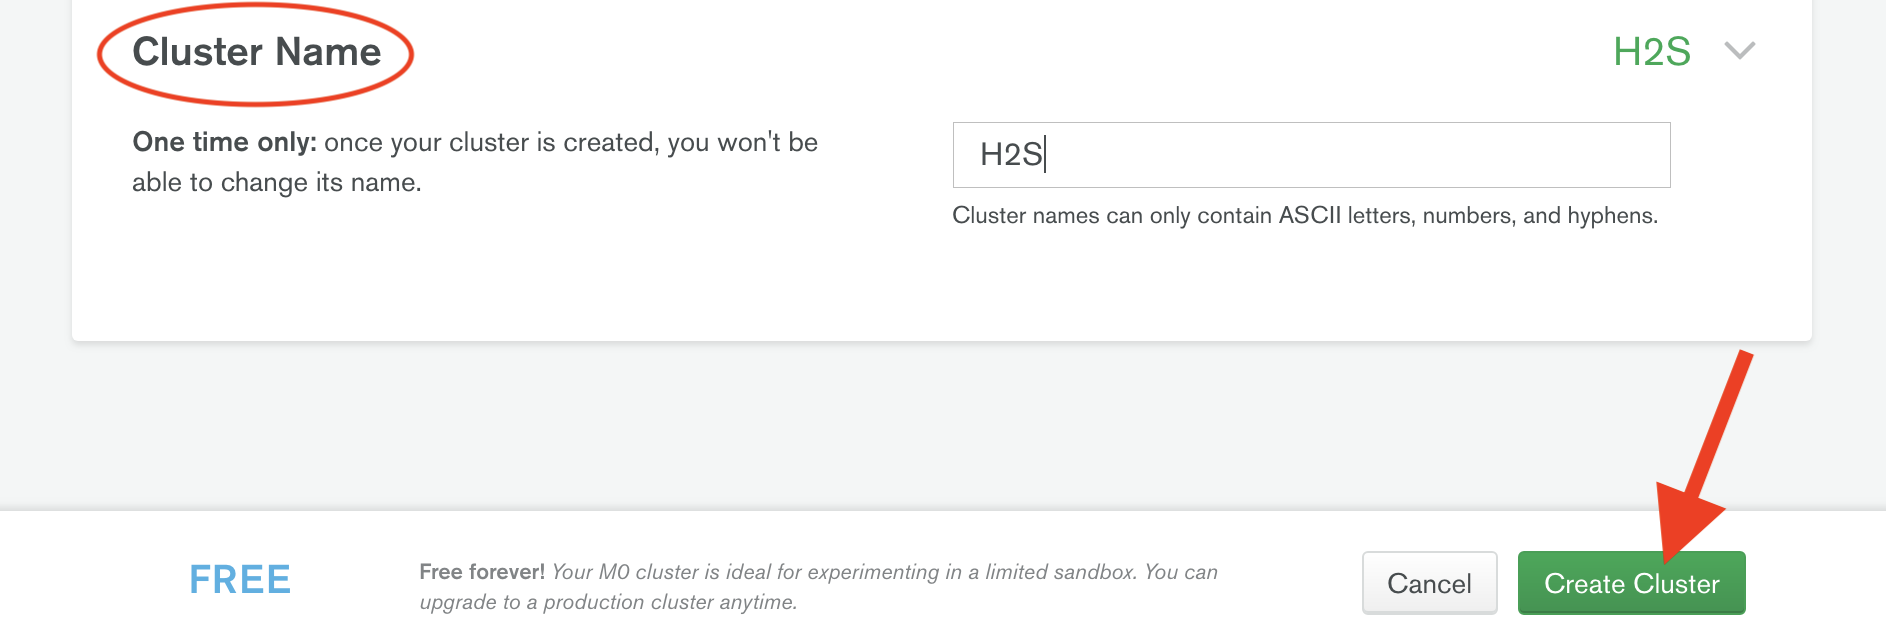
\includegraphics[width=14cm]{WEB/mongo_3.png}
    \end{center}
\end{figure}

\newpage
Now create your a database user
\begin{figure}[H]
    \begin{center}
        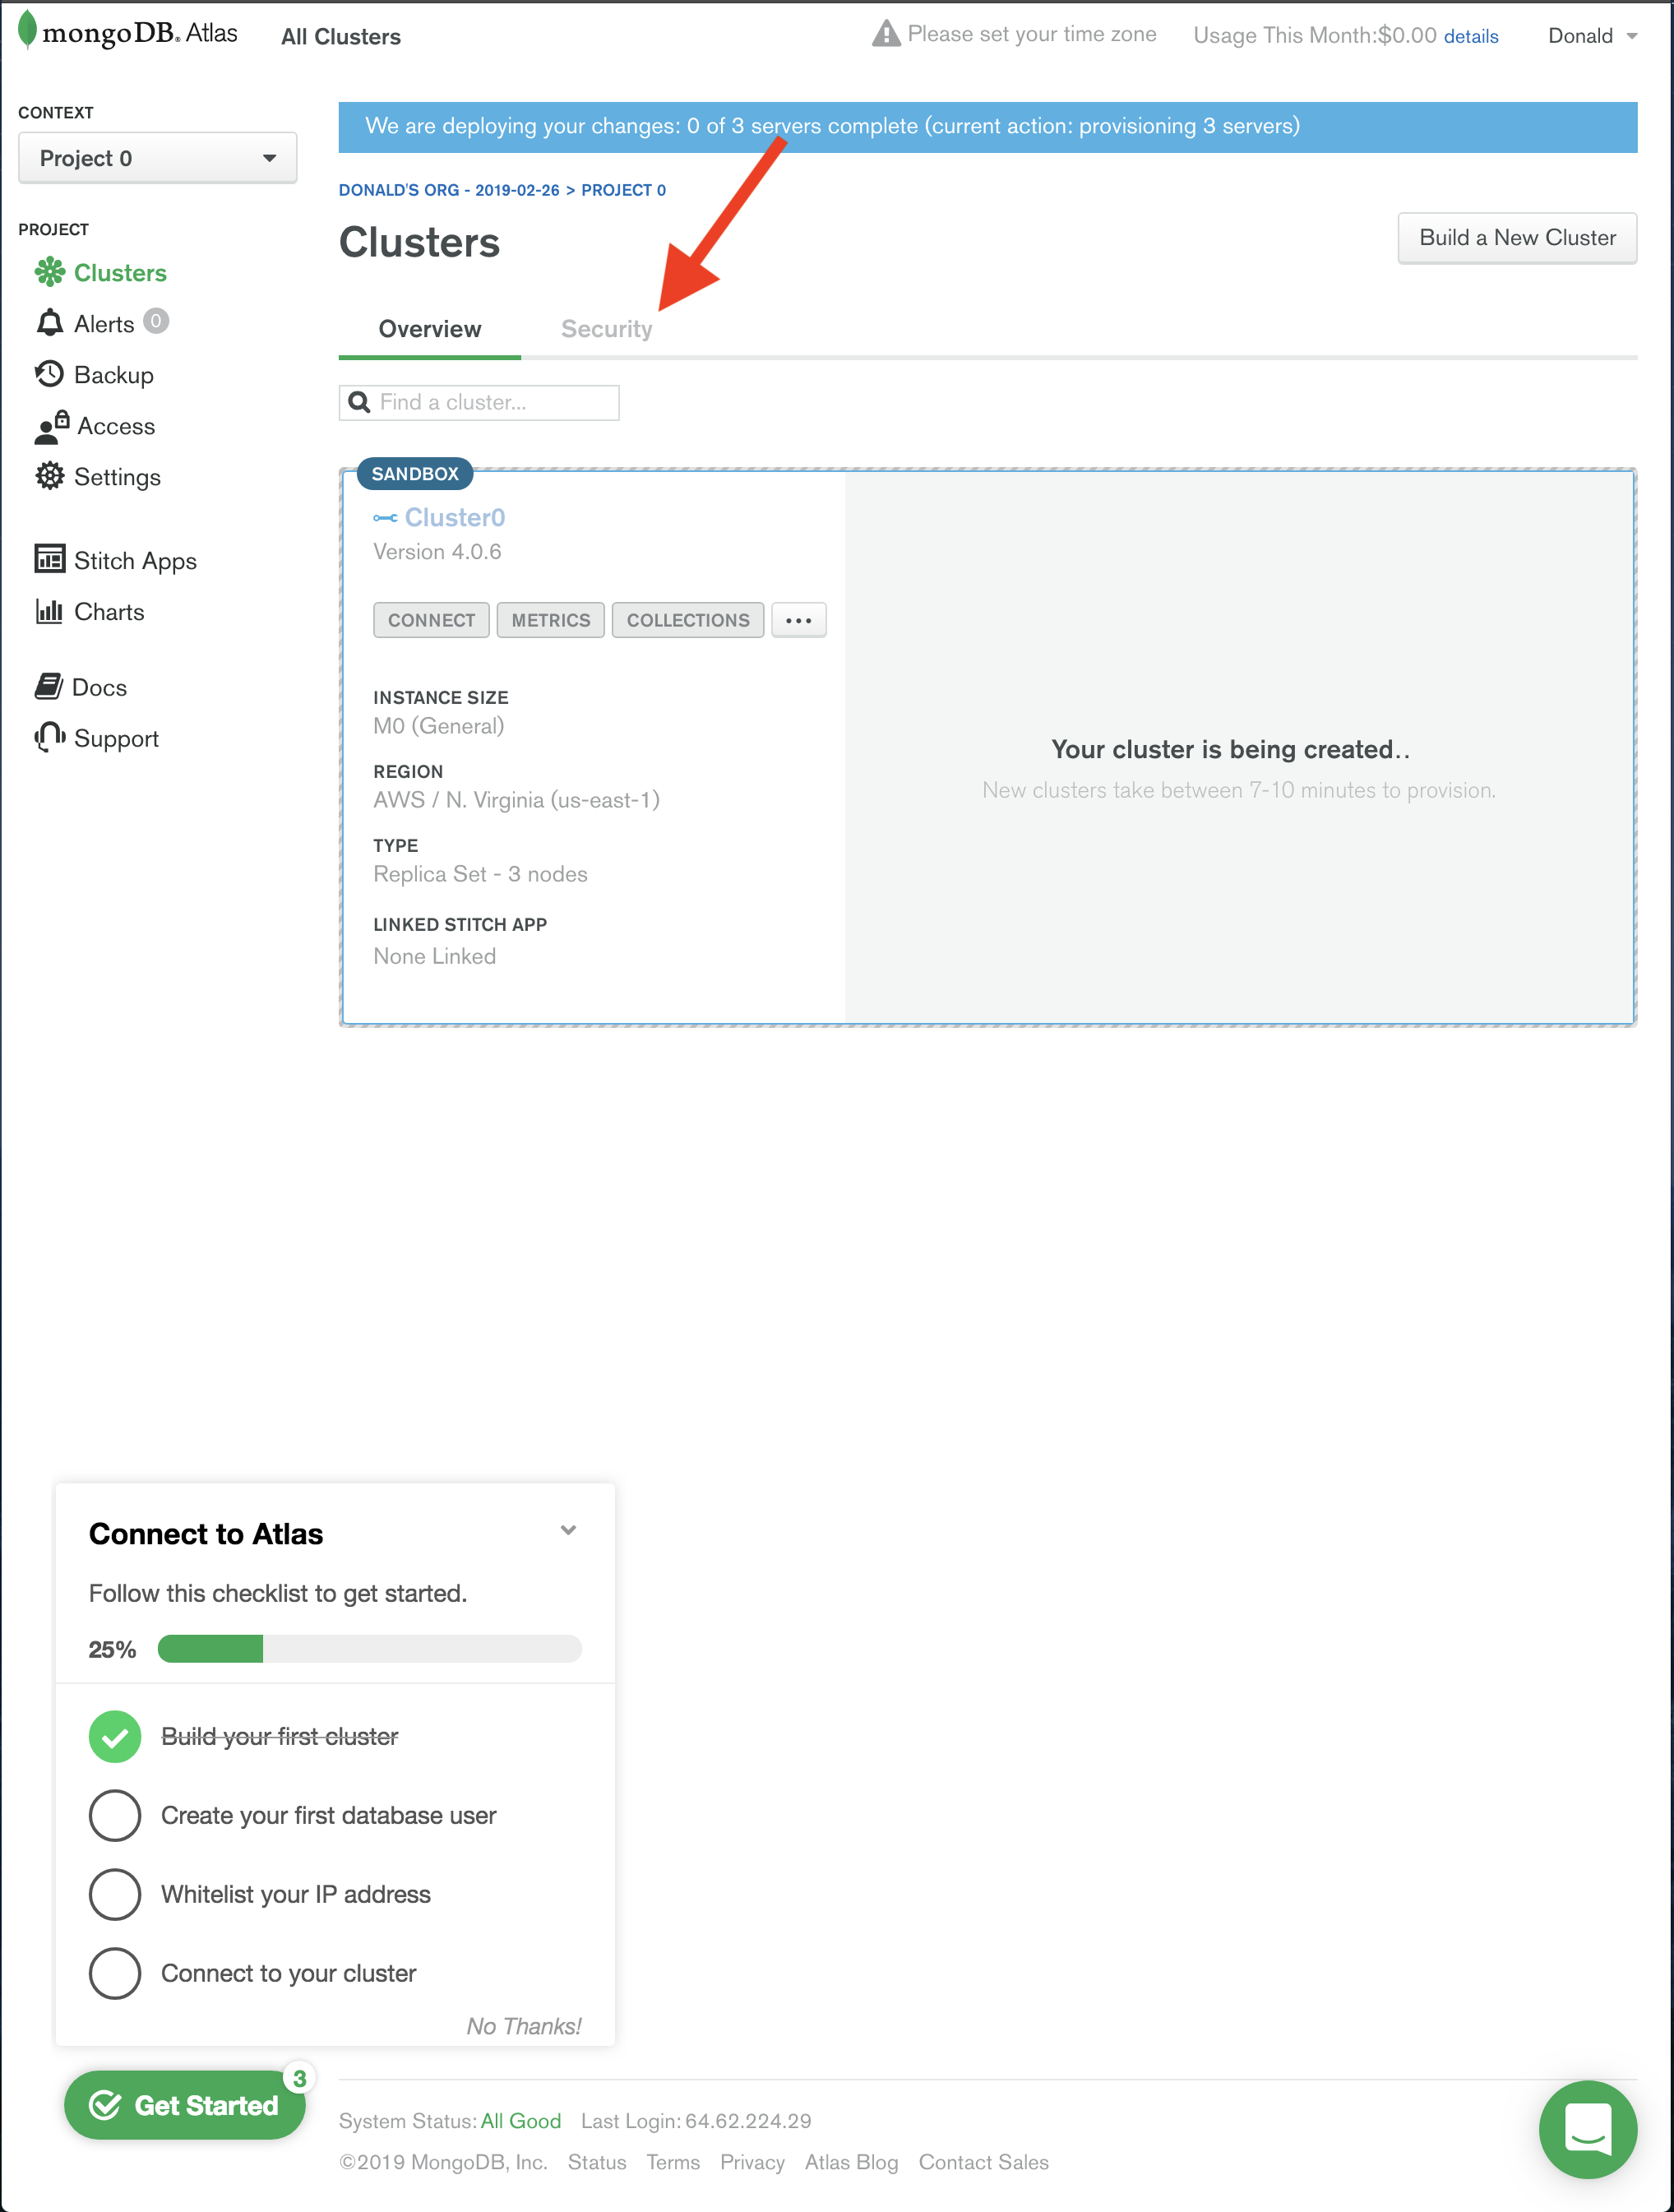
\includegraphics[width=14cm]{WEB/mongo_4.png}
    \end{center}
\end{figure}

\begin{figure}[H]
    \begin{center}
        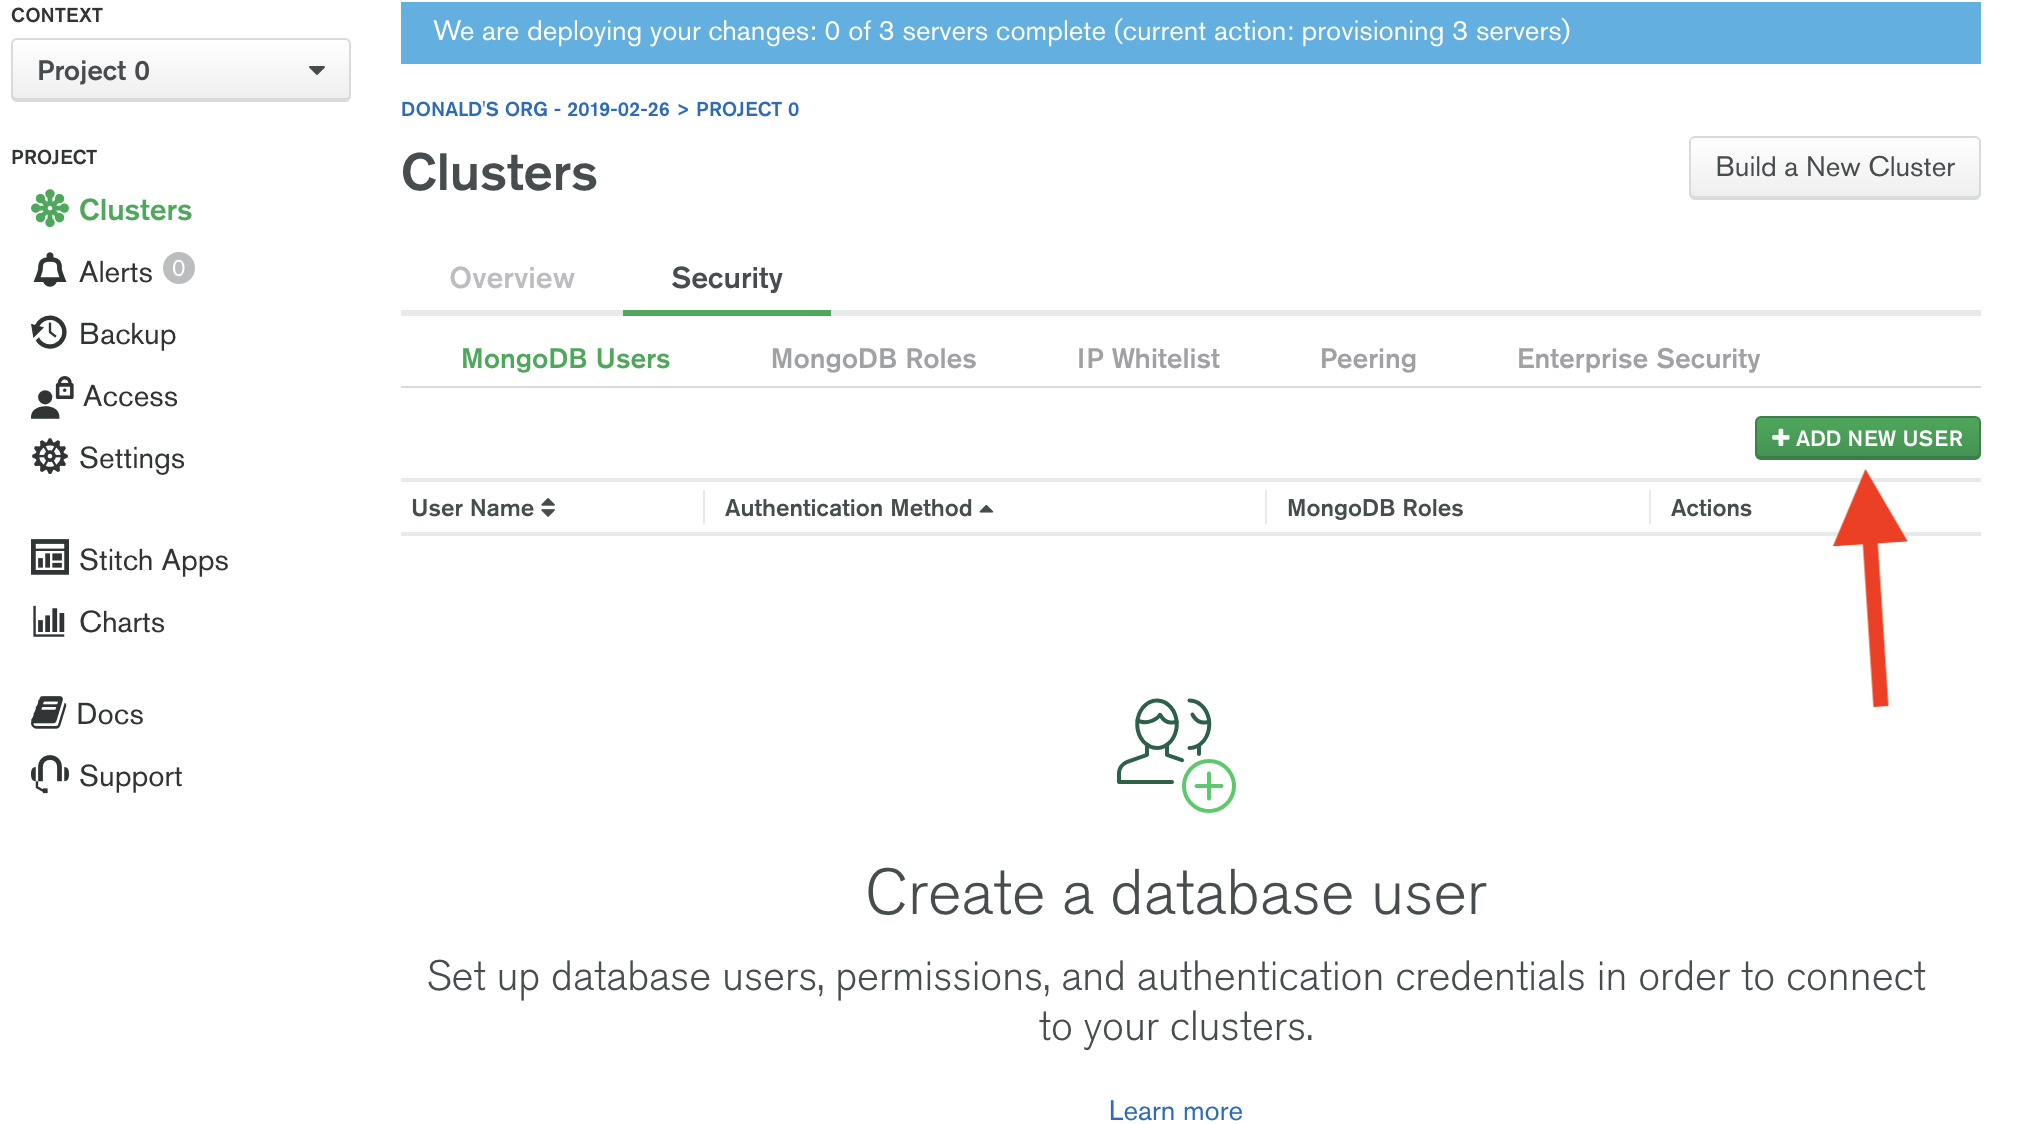
\includegraphics[width=14cm]{WEB/mongo_5.png}
    \end{center}
\end{figure}

\begin{figure}[H]
    \begin{center}
        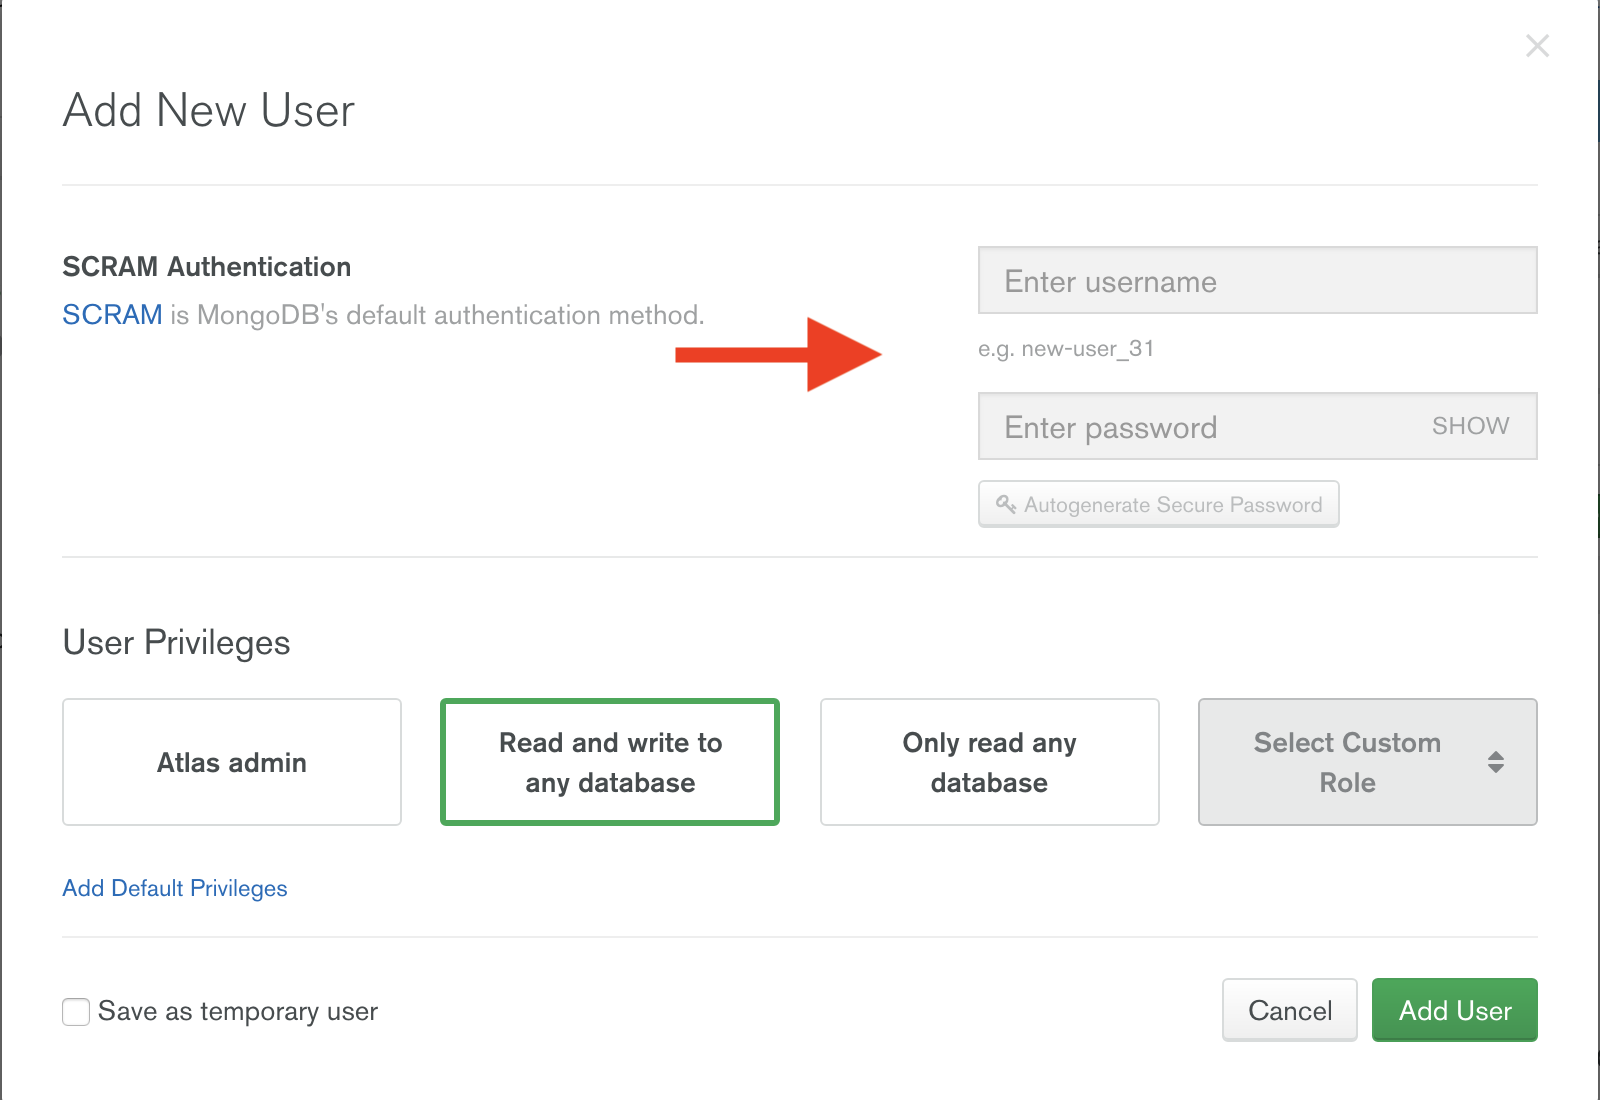
\includegraphics[width=14cm]{WEB/mongo_6.png}
    \end{center}
\end{figure}

\begin{figure}[H]
    \begin{center}
        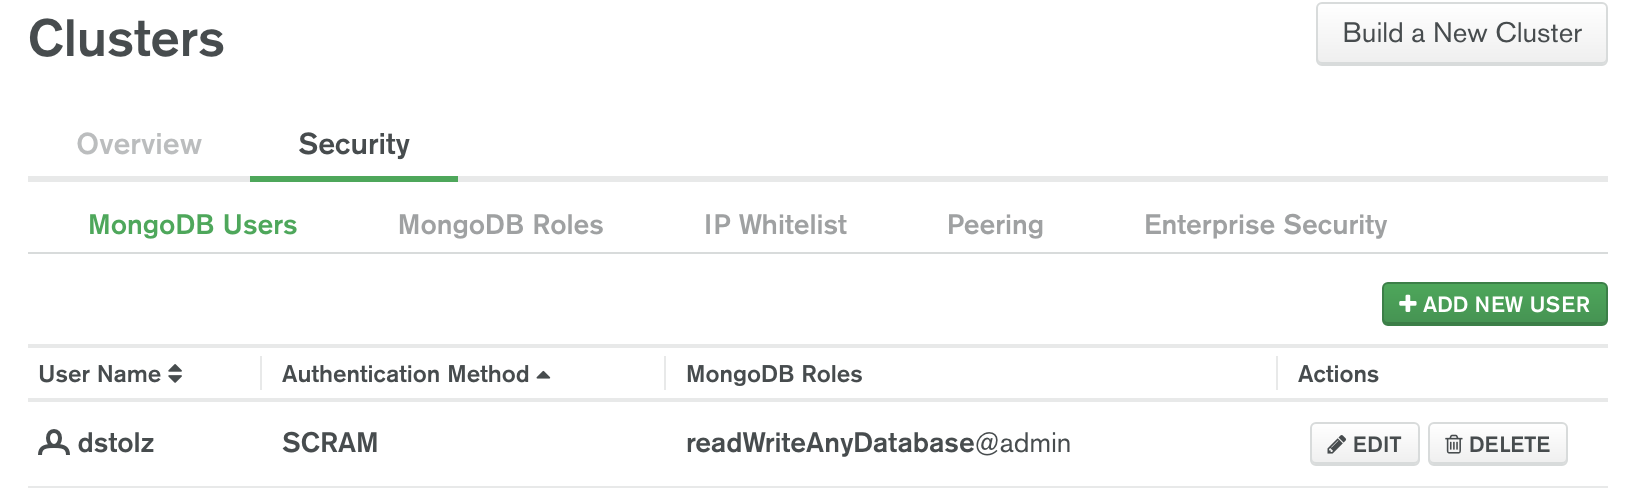
\includegraphics[width=14cm]{WEB/mongo_7.png}
    \end{center}
\end{figure}

\newpage
After creating a user you will need to whitelist your IP address
\begin{figure}[H]
    \begin{center}
        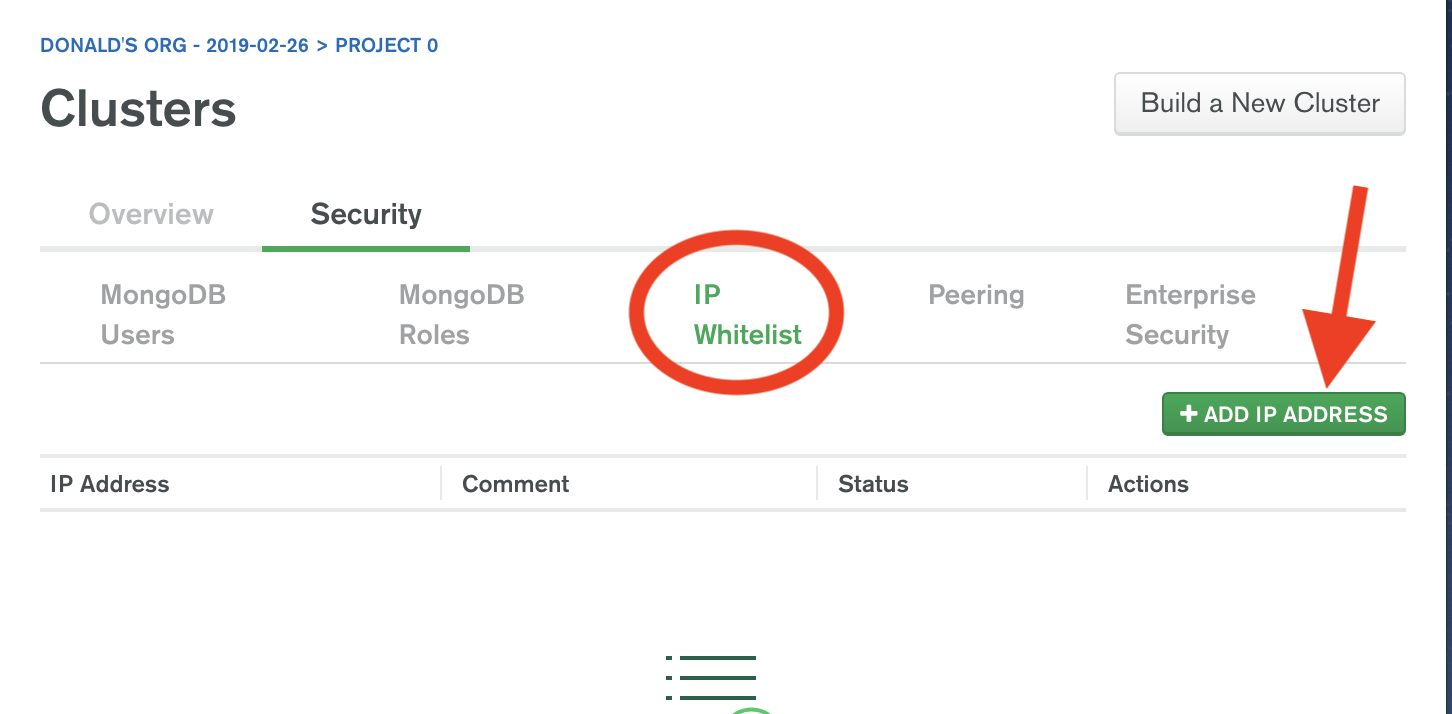
\includegraphics[width=14cm]{WEB/mongo_8.png}
    \end{center}
\end{figure}

\begin{figure}[H]
    \begin{center}
        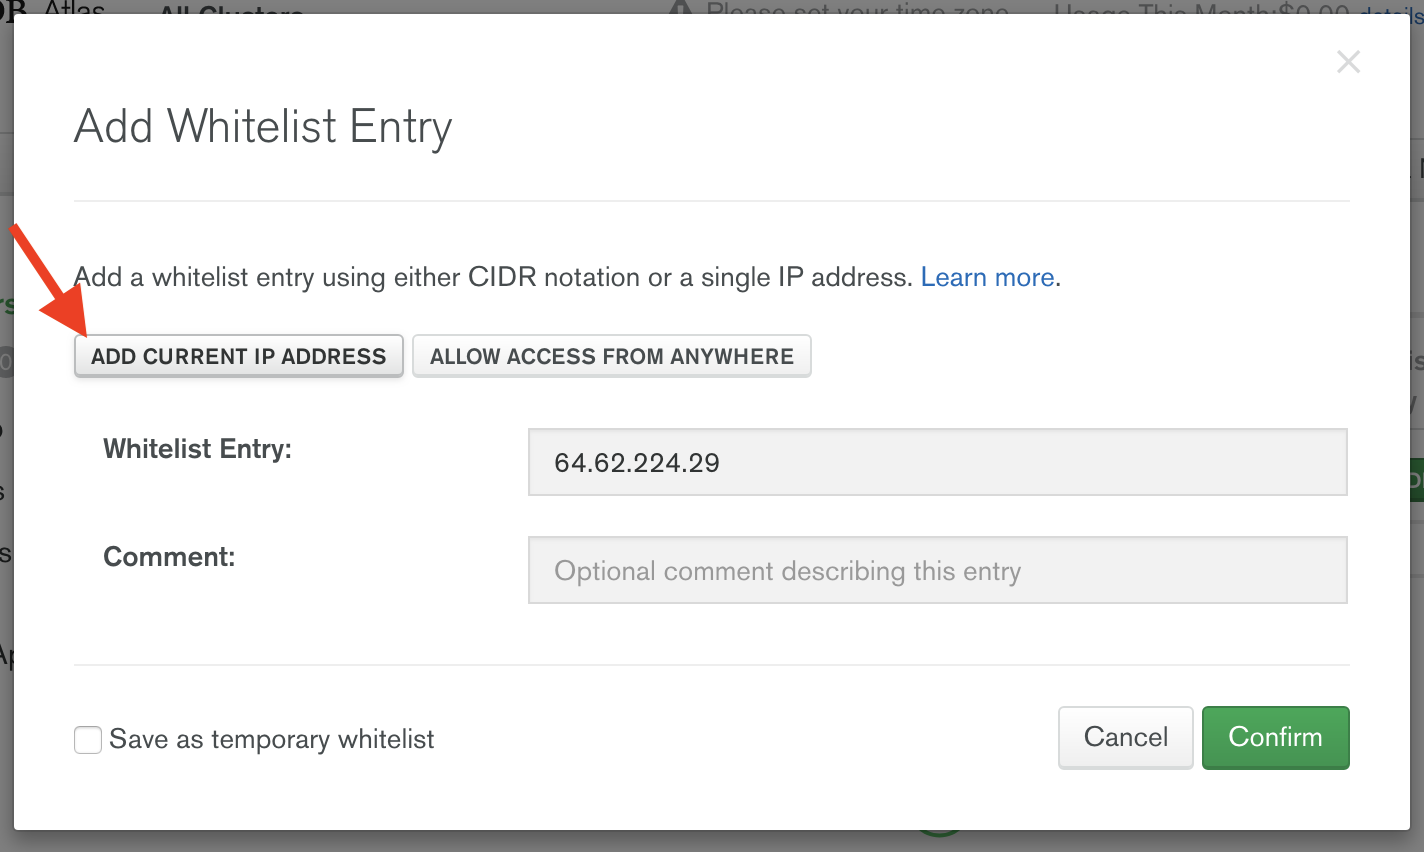
\includegraphics[width=14cm]{WEB/mongo_9.png}
    \end{center}
\end{figure}

\newpage
Once we have a user and our IP address is whitelisted we can get the address for connecting our app.
\begin{figure}[H]
    \begin{center}
        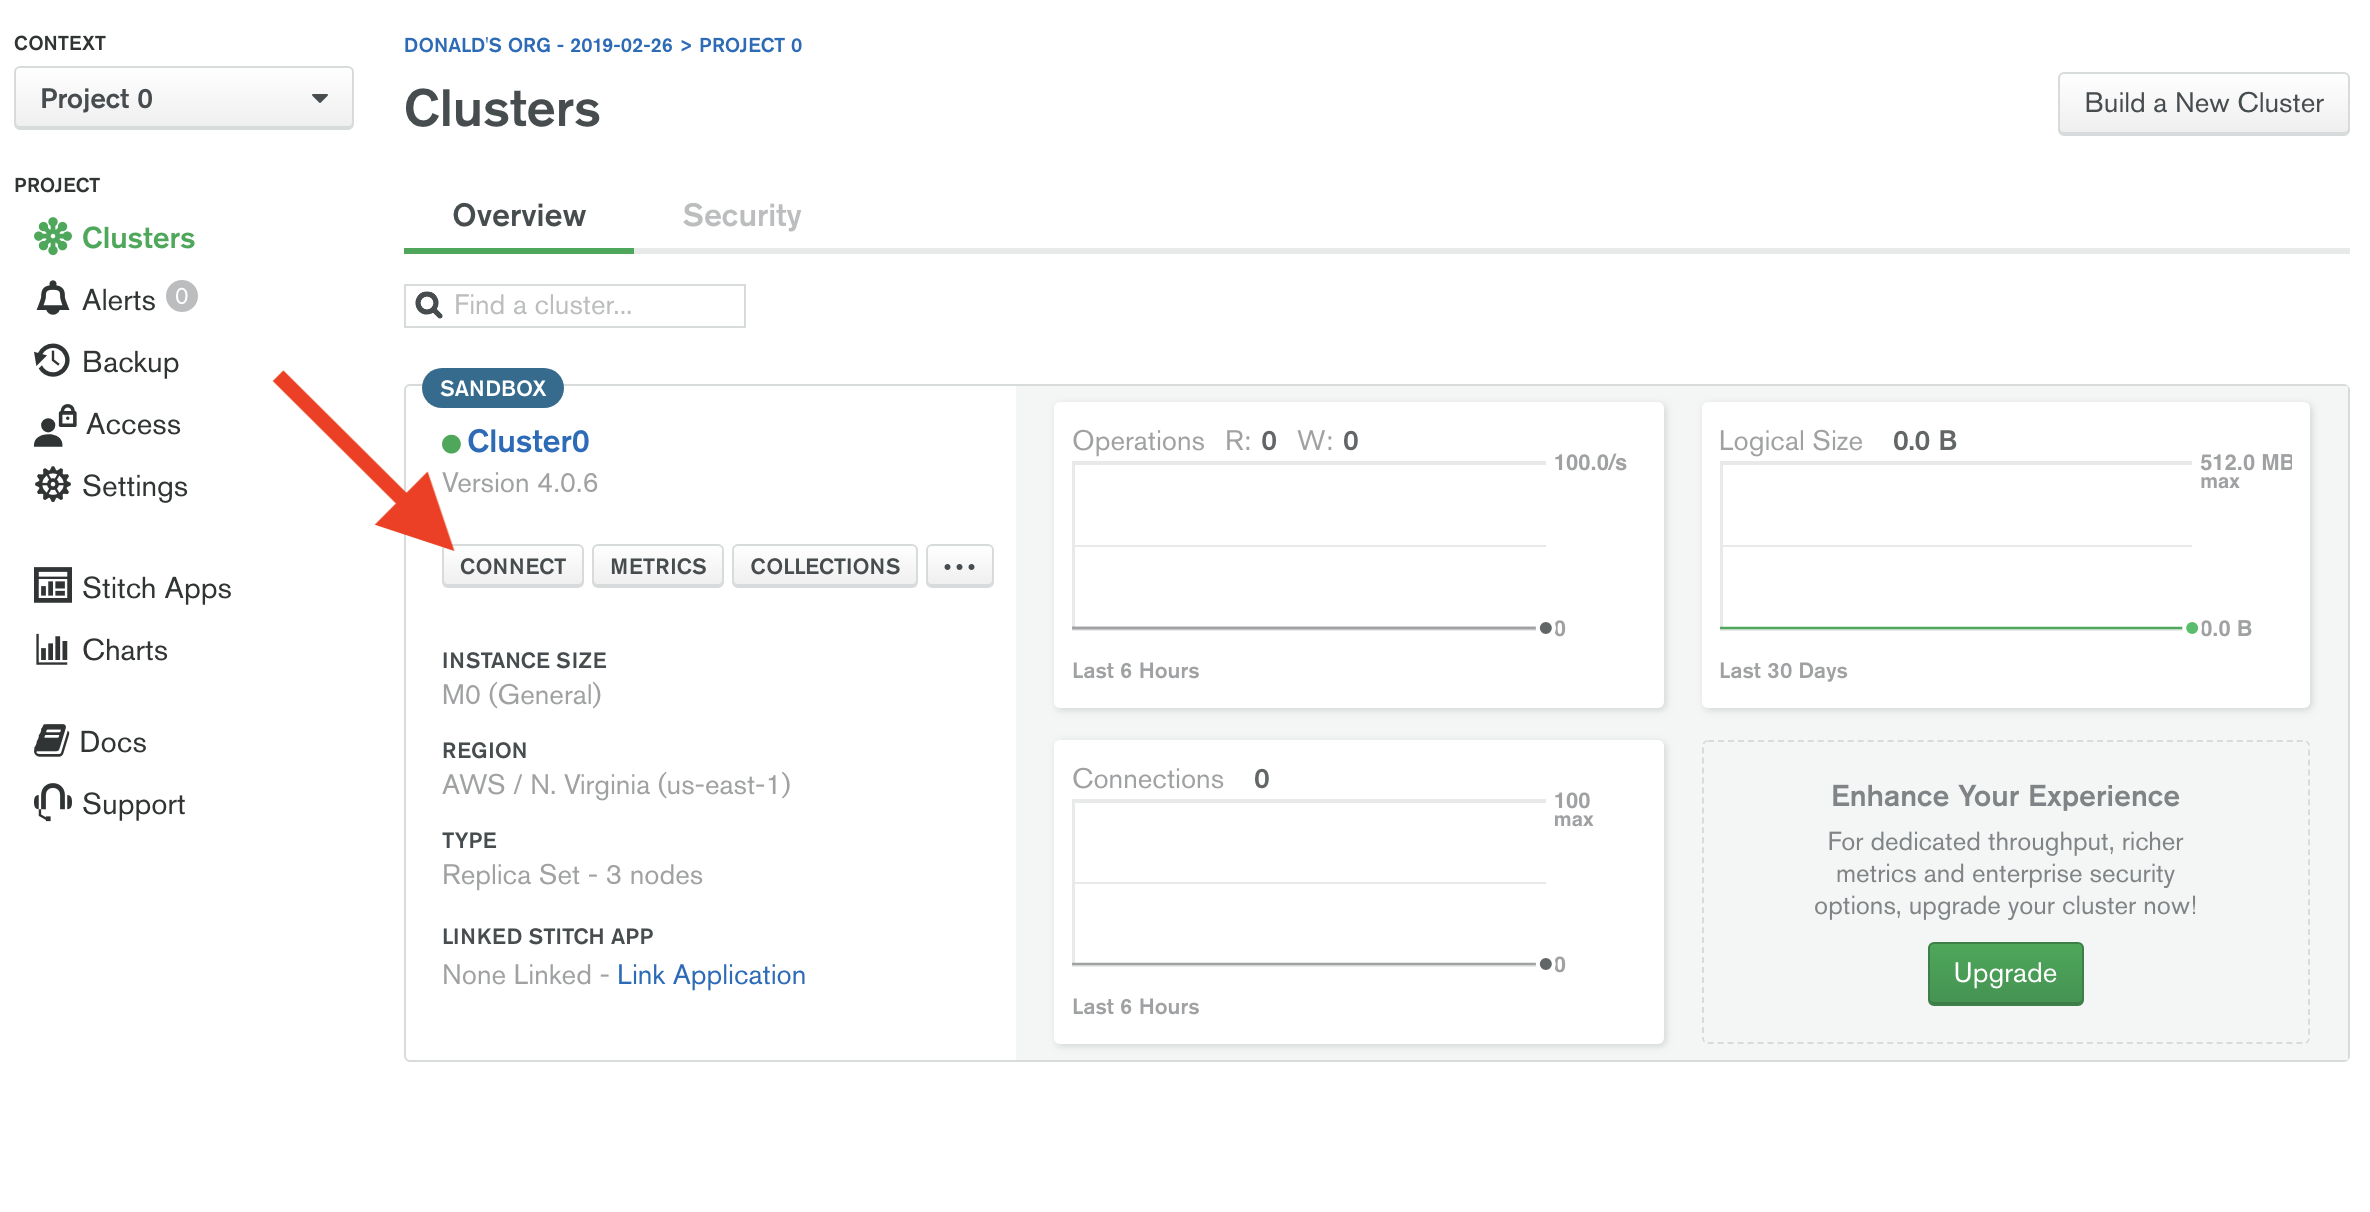
\includegraphics[width=14cm]{WEB/mongo_10.png}
    \end{center}
\end{figure}

\begin{figure}[H]
    \begin{center}
        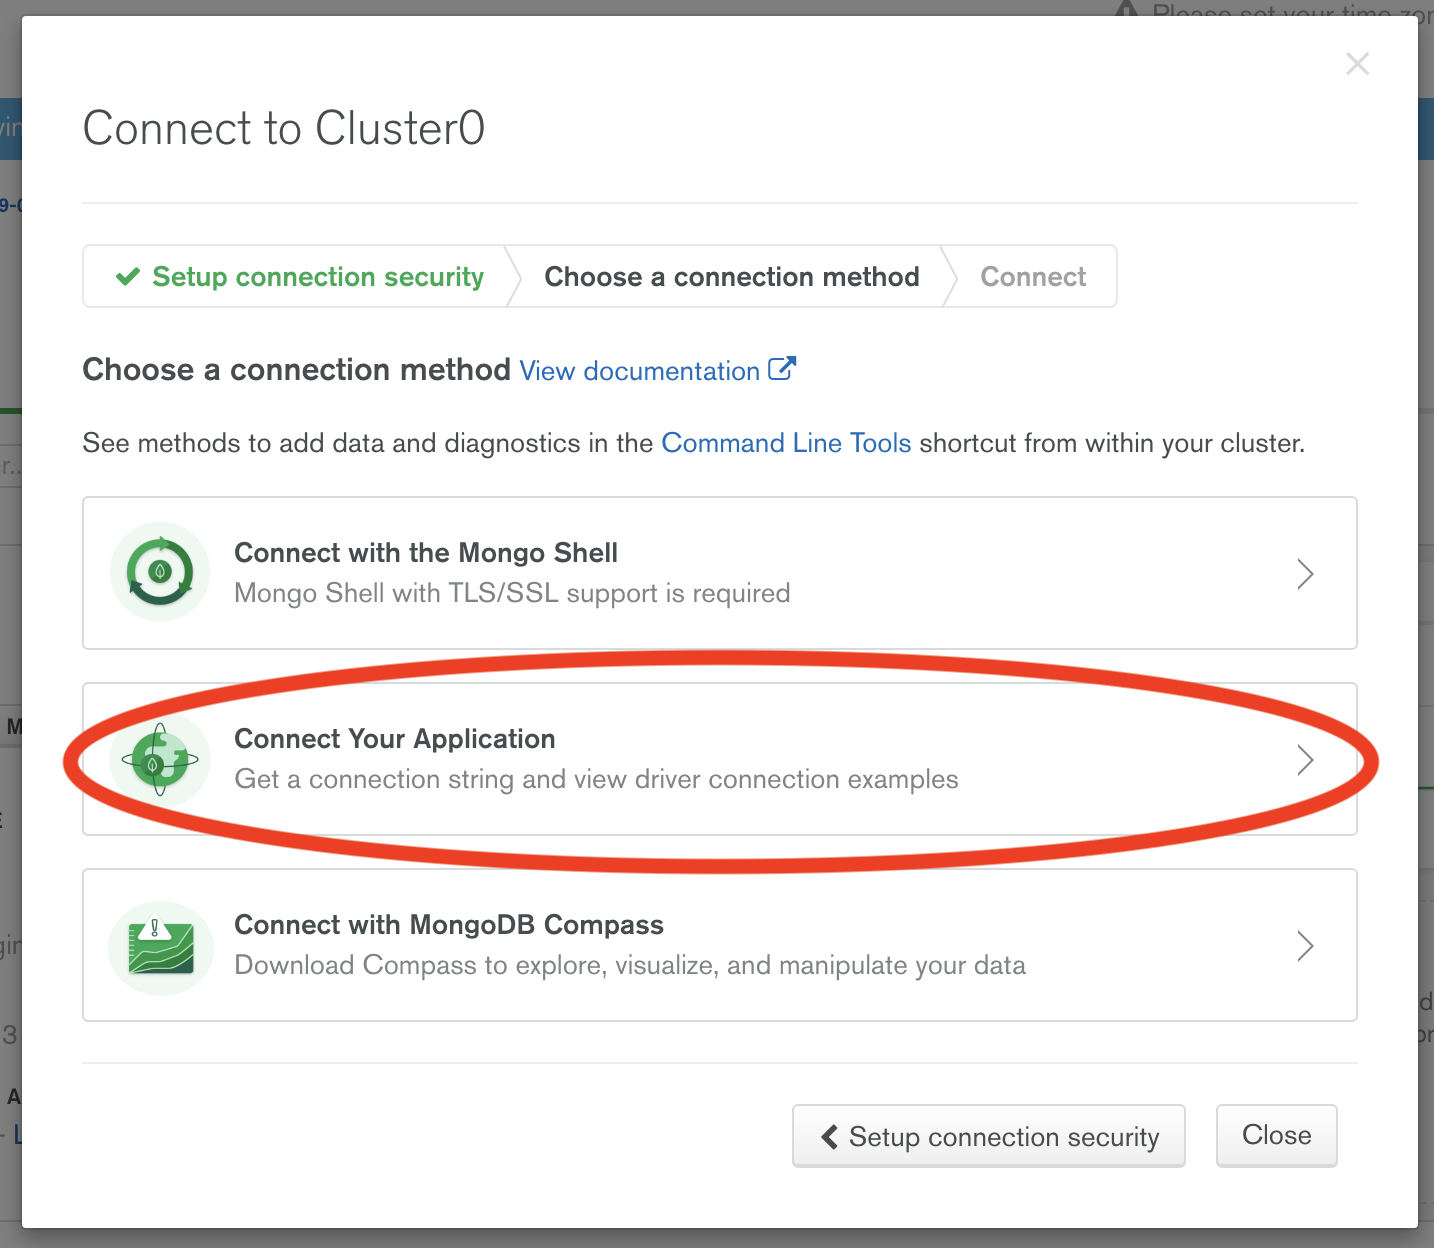
\includegraphics[width=14cm]{WEB/mongo_11.png}
    \end{center}
\end{figure}

\newpage
This is the address we will need for connecting to our database.
\begin{figure}[H]
    \begin{center}
        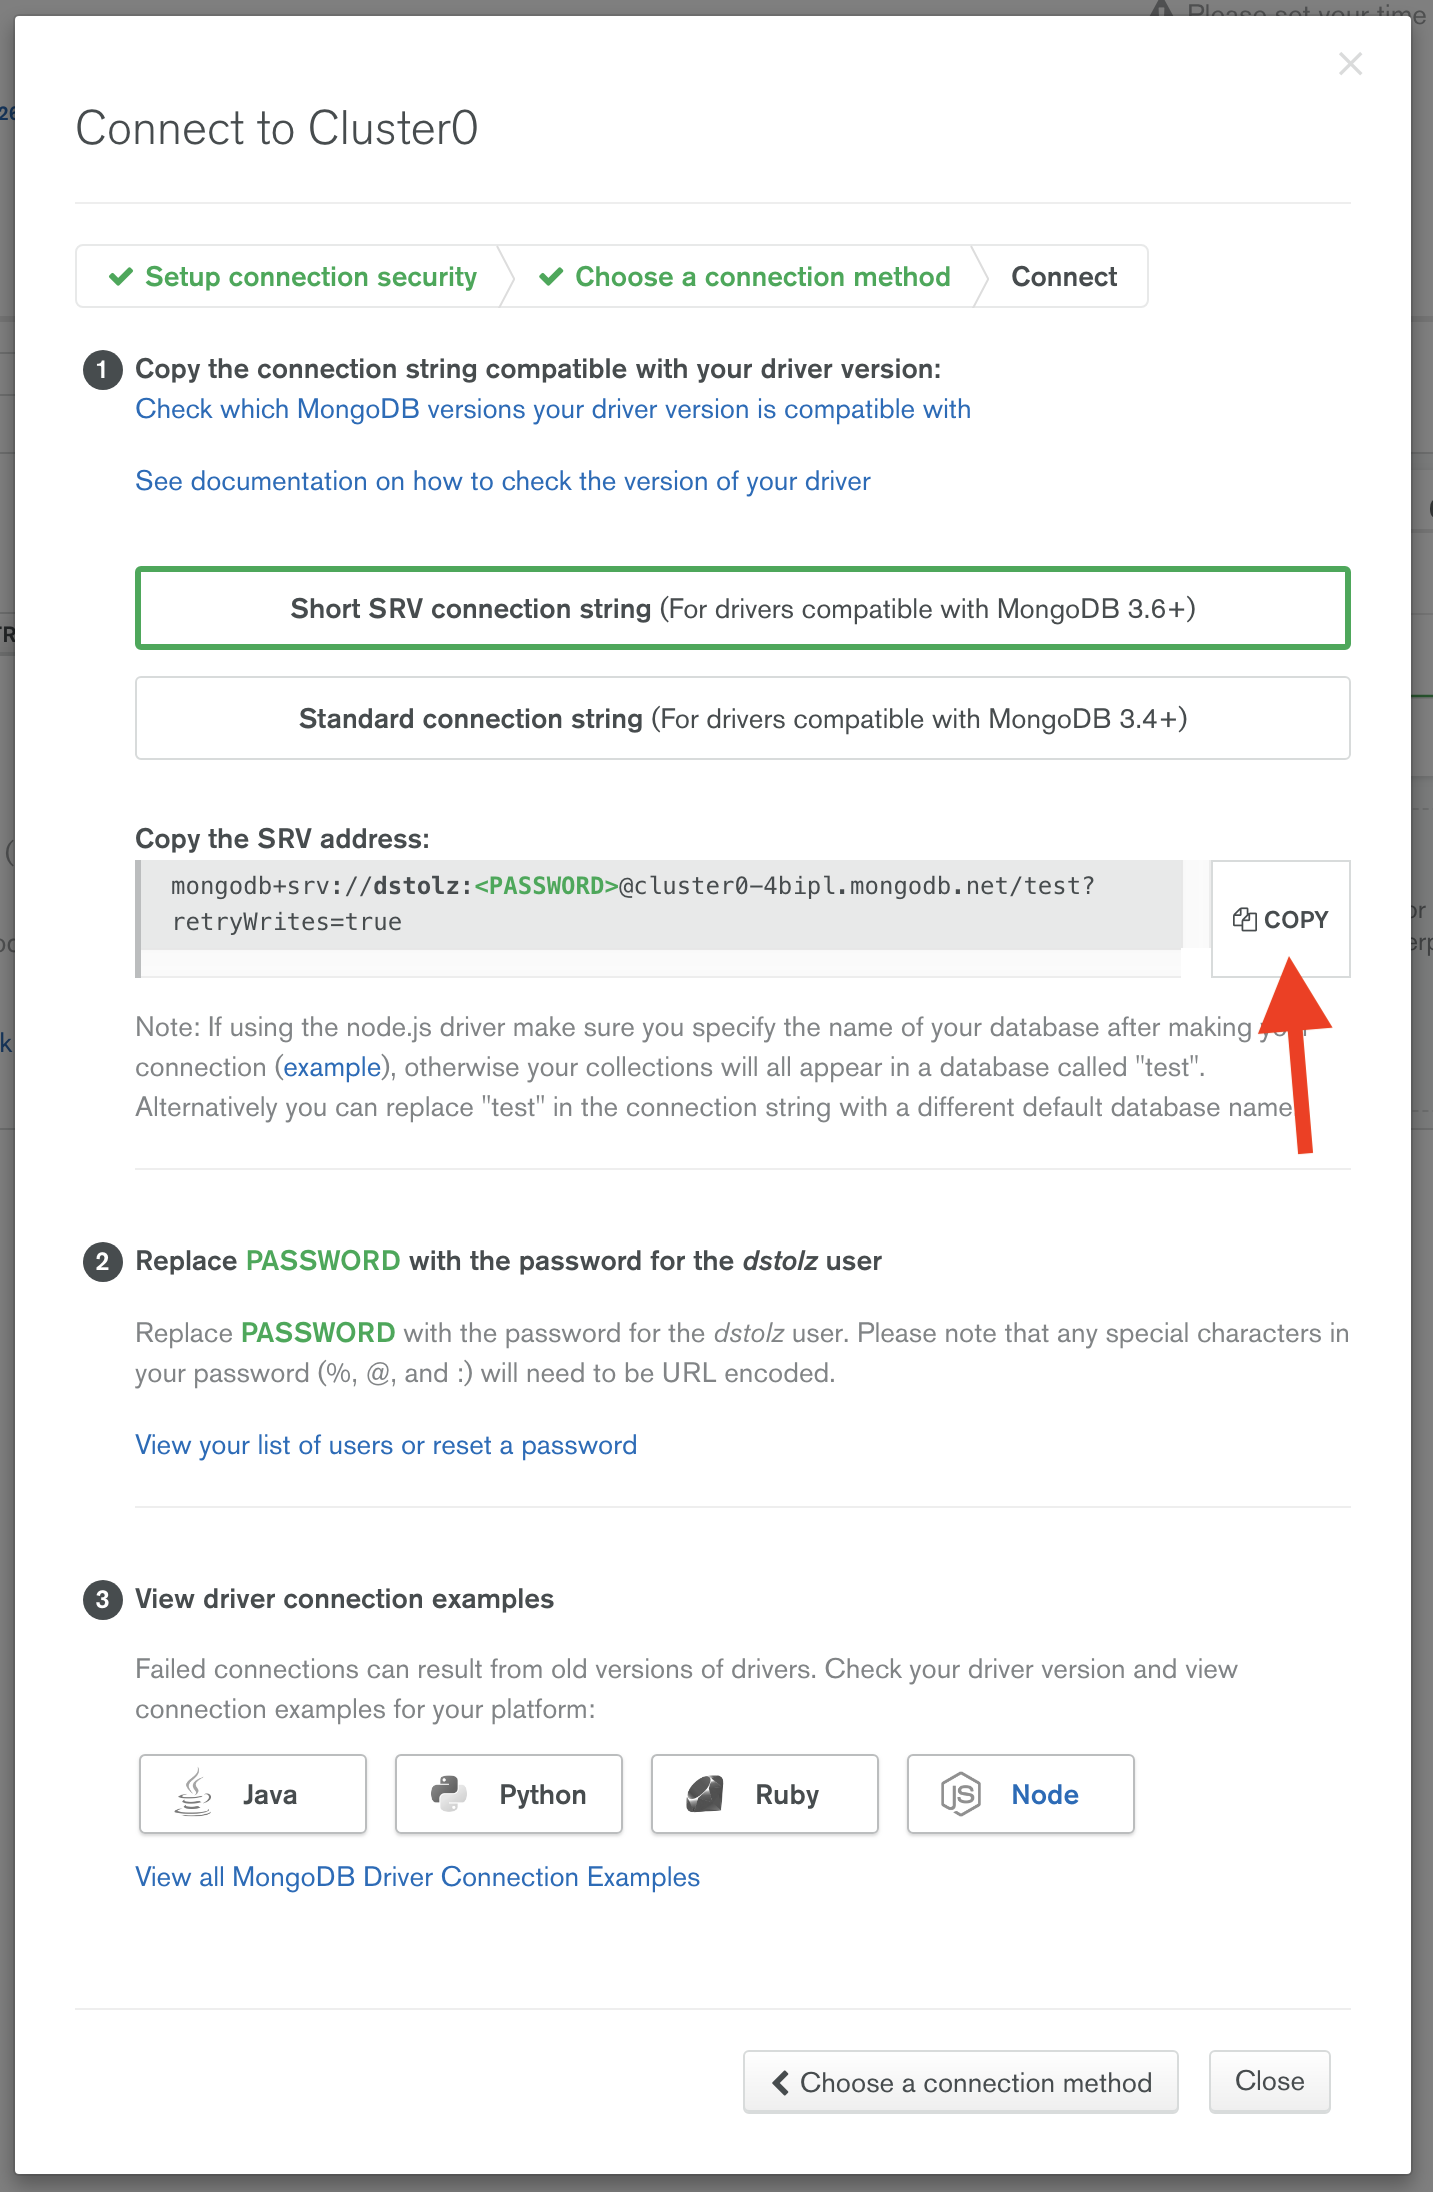
\includegraphics[width=14cm]{WEB/mongo_12.png}
    \end{center}
\end{figure}

%******************************************************************************%
\end{document}